\documentclass[12pt]{article}

\usepackage{background}     % Defining text colours.
\usepackage{enumitem}       % Better enumeration
\usepackage{fancyhdr}       % Headers and footers.
\usepackage[none]{hyphenat} % No hyphenation
\usepackage{multirow}       % Final table
\usepackage{parskip}        % Removes indentations from paragraphs.
\usepackage{xcolor}         % Coloured text.

% Setting dimensions
\newlength{\geometrytop}
\setlength{\geometrytop}{25pt}
\usepackage[papersize={12.8cm, 9.6cm},
            top=\geometrytop,
            headheight=15pt,
            headsep=5pt,
            bottom=0cm,
            marginparsep=0cm,
            marginparwidth=0cm,
            left=0.5cm,
            right=0.7cm,
            footskip=0cm]{geometry}

% Applying background.
\backgroundsetup{angle=0,
                 opacity=1,
                 position={21.6cm, -9.6cm},
                 scale=0.3,
                 contents={
\includegraphics{background.png}}}

% Set the font.
\renewcommand{\familydefault}{\rmdefault}
\renewcommand*\rmdefault{ppl}

% Defining font colours.
\definecolor{body}{rgb}{0.15, 0.15, 0.15}
\definecolor{bold}{rgb}{0.15, 0.15, 0.15}

% Defining text characteristics.
\newcommand{\body}[1]{{\color{body}#1}}
\newcommand{\embolden}[1]{{\bf\color{bold}#1}}
\newcommand{\slidetitle}[1]{~\\[-0.5ex]{\Large\bf{\color{bold}#1}}\\}

% Configuring header and footer, and removing horizontal header rule.
\pagestyle{fancy}
\fancyhf{}
\renewcommand{\headrulewidth}{0pt}

% Customise itemize environments.
\setitemize{itemsep=16pt, label=--, leftmargin=*}

% Configuring frameboxes for images.
\setlength{\fboxsep}{0cm}

\begin{document}

% Setting global font colour
\color{body}

% Begin
\thispagestyle{plain}
\begin{center}
\topskip0pt
\vspace*{\fill}
\LARGE{Python testing with pytest:\\[1ex]}
\Large{motivation, demonstration, and practices}
\normalsize
\vfill
Mark Vousden\\[5ex]
\vfill
\end{center}
\clearpage

%%%%%%%%%%%%%%%%%%%%%%%%% Introduction and why test? %%%%%%%%%%%%%%%%%%%%%%%%%

\begin{center}
\begin{tabular}{lr}
  \fbox{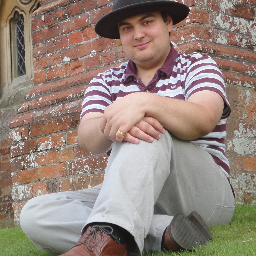
\includegraphics[width=0.32\textwidth]{mark.png}} &
  
\includegraphics[width=0.23\textwidth]{python.png}
\end{tabular}
\fbox{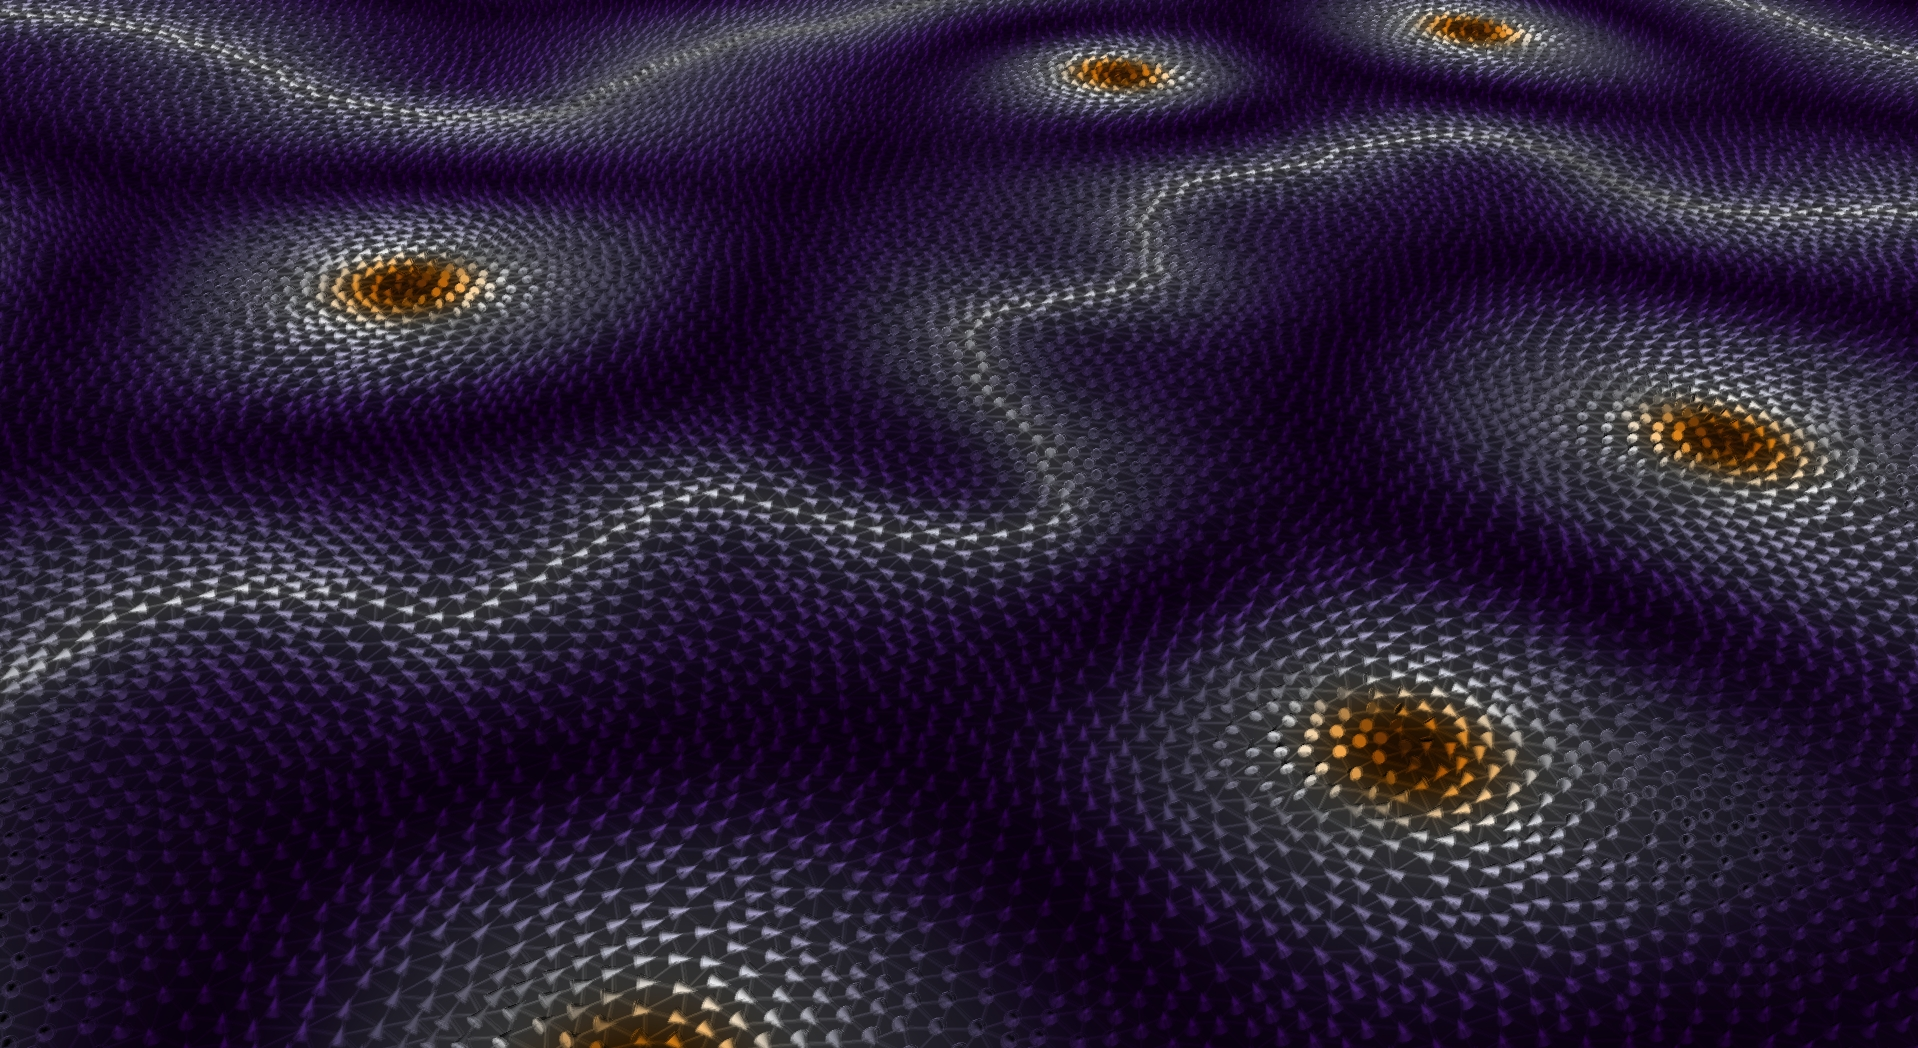
\includegraphics[width=0.6\textwidth]{hpc.png}}
\end{center}
\clearpage

\slidetitle{Why write tests?}
\begin{itemize}
\item Shows your software is fit for purpose
\item Do changes compromise your software?
\item Confidence!
\item Others can develop without risk
\end{itemize}
\clearpage

\slidetitle{Why {\color{red}not} write tests?}
\begin{itemize}[itemsep=-2.9pt]
\item Shows your software is fit for purpose
{\color{red} \item[] \hfill ``But I know it works!''}
\item Do changes compromise your software?
{\color{red} \item[] \hfill Takes time and skill}
\item Confidence!
{\color{red} \item[] \hfill False confidence!}
\item Others can develop without risk
{\color{red} \item[] \hfill Increased codebase (more to maintain)}
\end{itemize}
\clearpage

\thispagestyle{plain}
\vspace*{-\topskip}
\vspace*{\fill}
{\LARGE\centerline{Tests done badly are}
\centerline{worse than no tests at all.}}
\vspace*{\fill}
\vspace*{\geometrytop}
\clearpage

%%%%%%%%%%%%%%%% What should tests do? Outlining requirements %%%%%%%%%%%%%%%%

\slidetitle{Desirable features of a test suite}
\begin{itemize}
\item Shows the software is working or not (and failure diagnosis).
\item Test the software under many conditions (parameterisation).
% (without duplicating code)
\item Must run fast!
\item Test areas of software in isolation (mocking).
\item Many more...
\end{itemize}
\clearpage

\thispagestyle{plain}
\vspace*{-\topskip}
\vspace*{\fill}
{\Huge\centerline{\textbf{Scenario I}}~\newline
\centerline{A really complicated}
\centerline{simulation library}}
\vspace*{\fill}
\vspace*{\geometrytop}
\clearpage

\slidetitle{Summary of Scenario I}
\begin{itemize}
\item You can test your code without Pytest.
\item Pytest reports failed tests.
\item Pytest searches for tests for you.
\item Pytest has informative output.
\end{itemize}
\clearpage

\slidetitle{How did pytest do that?}
\begin{itemize}
\item Collection:
\begin{itemize}
\item Imports the test file.
\item Scans for functions and classes with \verb|test| in their handle.
\end{itemize}
\item Execution:
\begin{itemize}
\item Calls dependencies/fixtures (see scenario II).
\item Literally calls the test functions.
\end{itemize}
\end{itemize}
\clearpage

\thispagestyle{plain}
\vspace*{-\topskip}
\vspace*{\fill}
{\Huge\centerline{\textbf{Scenario II}}~\newline
\centerline{A data-processing library}}
\vspace*{\fill}
\vspace*{\geometrytop}
\clearpage

\slidetitle{Summary of Scenario II}
\begin{itemize}
\item Automatic test collection is useful.
\item Pytest shows us details about why assertions fail.
\item We need to be able to parameterise tests (without duplicating code).
\end{itemize}
\clearpage

\thispagestyle{plain}
\vspace*{-\topskip}
\vspace*{\fill}
{\Huge\centerline{\textbf{Scenario III}}~\newline
\centerline{A data-processing library}
\centerline{with parameterised tests}}
\vspace*{\fill}
\vspace*{\geometrytop}
\clearpage

\slidetitle{Summary of Scenario III}
\begin{itemize}
\item Fixtures (decorated with \verb|@pytest.fixture()|) are blocks of
    functionality that allow tests to be written in a modular way.
\item Fixtures are run when the test is run, and their output is passed to the
    test.
\item Fixtures can be used to parameterise tests, reducing code
    duplication. Each test is run individually of the others.
\item (Also, \verb|@pytest.mark.parameterize| can be used for this.)
\end{itemize}
\clearpage

\thispagestyle{plain}
\vspace*{-\topskip}
\vspace*{\fill}
{\Huge\centerline{\textbf{Scenario IV}}~\newline
\centerline{Sharing the load of}
\centerline{parameterised tests}
\centerline{(parallelisation)}}
\vspace*{\fill}
\vspace*{\geometrytop}
\clearpage

\slidetitle{Summary of Scenario IV}
\begin{itemize}
\item The \verb|pytest-xdist| pytest plugin allows tests to be distributed to
    other compute resources (typically local cores).
\item pytest can guess the number of cores you need (be careful).
\item Alternatively, make your software run in parallel, and use this to test
    serial regions.
\end{itemize}
\clearpage

\thispagestyle{plain}
\vspace*{-\topskip}
\vspace*{\fill}
{\Huge\centerline{\textbf{Scenario V}}~\newline
\centerline{Testing software in isolation}
\centerline{(mocking)}}
\vspace*{\fill}
\vspace*{\geometrytop}
\clearpage

\slidetitle{Test Types}
\vfill
\centerline{Isolation is not always appropriate.}
\vfill
\begin{tabular}{ccc}
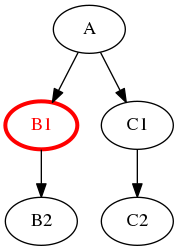
\includegraphics[width=0.3\textwidth]{unit.png} &
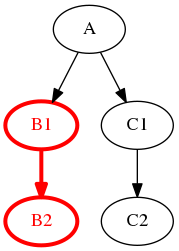
\includegraphics[width=0.3\textwidth]{integ.png} &
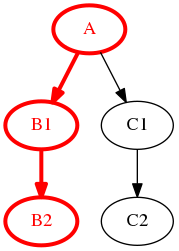
\includegraphics[width=0.3\textwidth]{sys.png} \\
Unit tests & Integration tests & System tests
\end{tabular}
\vfill
\vfill
\clearpage

\slidetitle{Summary of Scenario V}
\begin{itemize}
\item Mocking (we used \verb|pytest-mock|) allows you to live-swap one imported
    function with another.
\item We can test individual behaviours of complicated functions.
\item Unit tests, integration tests, and system tests all serve different
    purposes; mocking helps with these.
\item (Beware of parallel file input/output!)
\end{itemize}
\clearpage

\slidetitle{Other useful testing-related tools}
\begin{itemize}[itemsep=0cm]
\item Other testing frameworks like \verb|unittest| or \verb|nose|.
\item \verb|pytest-timeout| to catch timeouts.
\item \verb|pdb| (or \verb|ipdb|) is a debugger that can be used during
    tests. \verb|--pdb| flag starts python debugger on collection error.
\item \verb|pytest-cov| for code coverage.
\item Version control and continuous integration (CI).
\item Git bisect
\item \verb|--junitxml| dumps a machine-readable XML of results.
\item \verb|conftest.py| to configure collection behaviour.
\end{itemize}
\clearpage

\slidetitle{Summary}
\begin{itemize}
\item Testing software is often essential.
\item Writing tests is hard. Bad tests are harmful!
\item There are many approaches, but pytest is good.
\item The testing rabbit hole is deep.
\end{itemize}
\clearpage

\slidetitle{Closing}\\[0.5cm]
Get pytest at www.pytest.org (use pip or conda!)
\vfill
\renewcommand{\arraystretch}{1.2}
\begin{tabular}{ll}
\multirow{2}{*}{
\includegraphics[width=1cm]{github.png}} &
Presentation: mvousden/pytest-spug-2017 \\
& Code examples: mvousden/pytest-lets-explore \\
\multirow{2}{*}{
\includegraphics[width=1cm]{email.png}} &
\multirow{2}{*}{mlvousden@gmail.com} \\ \\
\multirow{2}{*}{
\includegraphics[width=1cm]{youtube.png}} &
\multirow{2}{*}{Link coming soon!} \\ \\
\end{tabular}
\vfill
\clearpage

\end{document}
